\chapter{From Compressibility to Light Refraction}
\label{chapter: Theory}

\par A brief theoretical background is needed to understand how the relationship between compressibility and refraction culminate on optical flow visualization techniques. The next subsections will first explain how high speeds give rise to density changes in a fluid. It will highlight the importance of the Mach Number, give a description of compression and expansion waves, and how it can be applied in real cases such as compressible jets and aerospikes nozzles. Afterwards it will treat on refraction, stressing the most important aspects that make Schlieren imaging possible.
% Finally, a detailed description of the schlieren-based methods is given, finishing with laser speckled BOS and the research gap. 

\section{Compressibility and Density}
\label{section: Compressibility}

\par The ability of fluid to change its density is called compressibility. Air is a gas mixture, so its molecules are distanced enough that they are able to move closer together when some pressure is applied. Due to this, air is classified as having high compressibility. When objects move slowly through it, changes in pressure throughout the flow field are small enough that the effect can be neglected as an engineering approximation, and density can be assumed constant. This is the incompressible assumption, and it can be expressed through the relation between density $\rho$ and pressure p via the compressibility coefficient $\tau$, as shown in the equation: $d \rho =\rho \tau dp$.

\par When high speeds are achieved, the pressure gradients through the flow field become larger, leading to a significant change in density that needs to be accounted for. A normal threshold for compressible flows is when the Mach Number ($M$) surpasses 0.3, which marks the point where density changes are higher than $5\%$ \cite{TheBookOfAnderson}. The Mach number is a non-dimensional quantity, defined by Equation \ref{equation:Mach Number}, that governs the behavior of waves traveling faster than the speed of sound. This behavior was discovered in 1885 by Ernst Mach and Wentzel when working on such structures with schlieren imaging \cite{Settles2001}.

\begin{equation}
    \label{equation:Mach Number}
    M = \frac{V}{a}
\end{equation}

These supersonic waves were described before by Riemann, and they form when an object moves faster than the sound waves emitted by it. This makes the sound waves pile up and coalesce, forming a standing wave in front of the body \cite{TheBookOfAnderson}, as illustrated in Figure \ref{fig: Moving sound wave}. 

\begin{figure}[htbp]
    \centering
    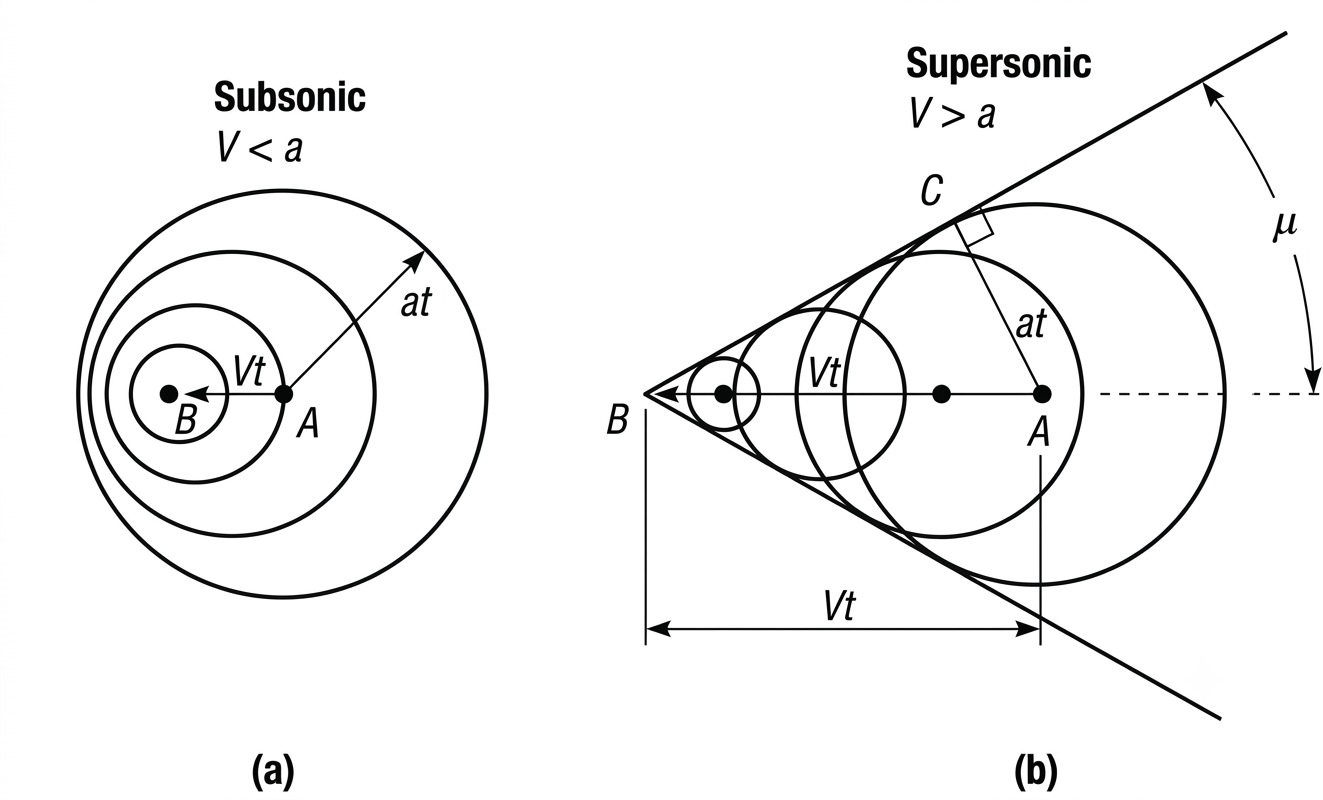
\includegraphics[width=0.5\textwidth]{figures/Moving sound waves.png}
    \caption{Propagation of information by an object moving at (a) subsonic speeds and (b) supersonic speeds, credit to Anderson \cite{TheBookOfAnderson}}
    \label{fig: Moving sound wave}
\end{figure}

Figure \ref{fig: Moving sound wave} shows an object leaving point A at a speed faster than the speed of sound, after a time interval $t$ it has traveled $Vt$, while the first emitted wave has only propagated a distance $at$. A supersonic wave is created tangentially to the emitted sound waves and has an oblique angle $\mu$ called the Mach Angle. The picture allows us to make the following geometric relationship:
\begin{equation}
    \sin \mu = \frac{a t}{V t} = \frac{1}{M}
\quad \Leftrightarrow \quad
\mu = \arcsin\!\left(\frac{1}{M}\right)
\end{equation}

\par The coalescence of the emitted waves creates an extremely thin region (of around $10^{-7}$m of magnitude) where the flow properties change drastically, in an almost explosive compression process that originates a seemingly discontinuous pressure increase across it \cite{TheBookOfAnderson}. When the emitted sound from the object becomes stronger, an oblique shock wave with an angle $\beta$ from the freestream air is formed, where $\beta > \mu$. Through this oblique shock wave, the pressure, density, temperature and entropy of the flow increases, while the total pressure, Mach number and velocity decreases. These relationships are described by the continuity, momentum and energy equations for oblique shocks, summarized by Equation \ref{equation: oblique continuity}, \ref{equation: oblique momentum} and \ref{equation: oblique energy} respectively, given the geometry of Figure \ref{fig: Oblique shock geometry}.

\begin{figure}[htbp]
    \centering
    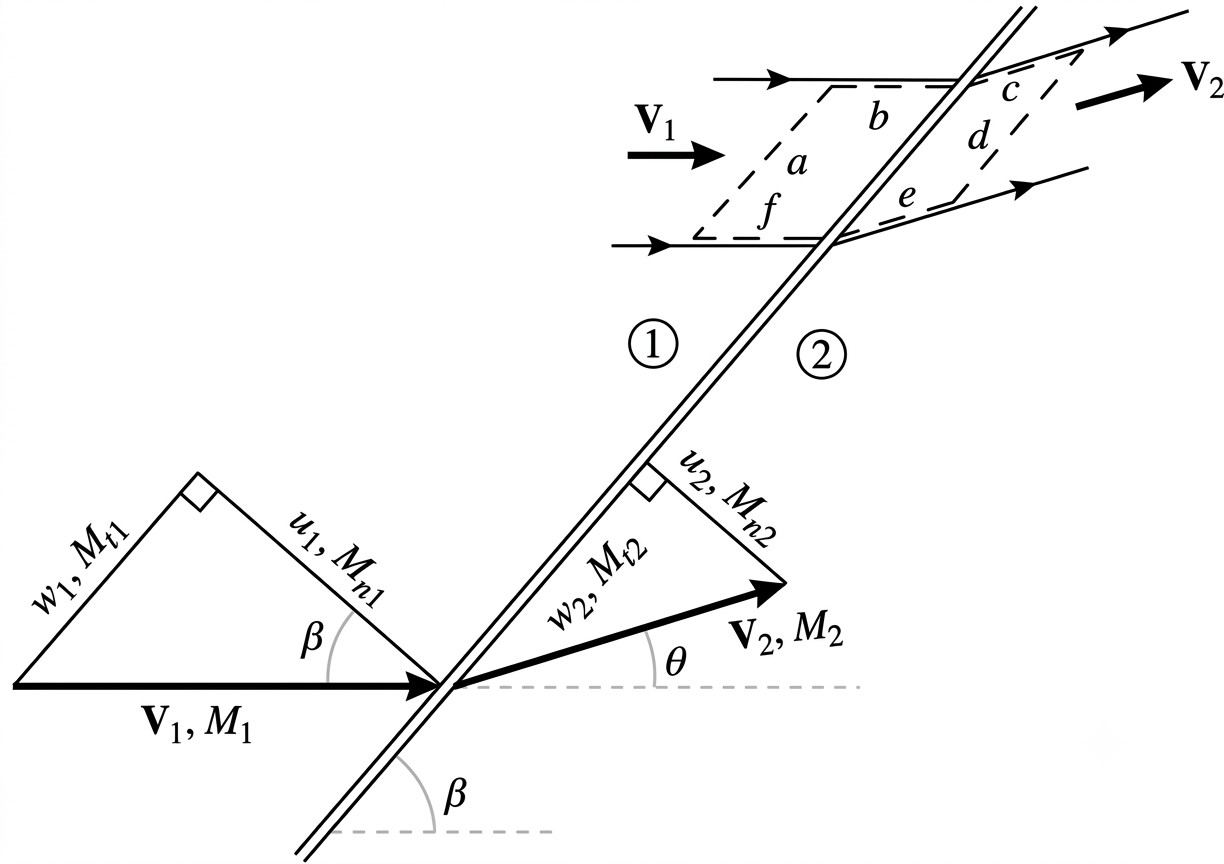
\includegraphics[width=0.5\textwidth]{figures/Oblique shock geometry.png}
    \caption{Oblique shock geometry, credit to Anderson \cite{TheBookOfAnderson}}
    \label{fig: Oblique shock geometry}
\end{figure}

\begin{align}
\rho_1u_1 &= \rho_2u_2 \label{equation: oblique continuity} \\
p_1 + \rho_1 u_1^2 &= p_2 + \rho_2 u_2^2 \label{equation: oblique momentum} \\
h_1 + \frac{u_1^2}{2} &= h_2 + \frac{u_2^2}{2} \label{equation: oblique energy}
\end{align}

\par These equations relate the flow properties before and after the shock. It is important to note that these changes depend only on the velocity component normal to the shock, with the tangential component maintaining constant. Considering a calorically perfect gas and adiabatic flow across the shock, it is possible to obtain the following relationships for $M_2, \rho_2$ and $p_2$ that rely only on $M_1$ and $\beta$.

\begin{align}
M_{n,1} &= M_1 \sin\beta, \\
 M_{n,2} &= M_2\sin(\beta-\theta)\\ 
M_{n,2}^{2}
&=
\frac{1 + M_{n,1}^{2}(\gamma - 1)/2}
{\gamma M_{n,1}^{2} - (\gamma - 1)/2}, \\
\frac{\rho_2}{\rho_1}
&=
\frac{(\gamma + 1)M_{n,1}^{2}}
{2 + (\gamma - 1)M_{n,1}^{2}}, \\
\frac{p_2}{p_1}
&=
1 + \left(\frac{2\gamma}{\gamma + 1}\right)
\left(M_{n,1}^{2} - 1\right).
\end{align}

\par These are important equations, as they allow the computation of the conditions after the shock by only knowing the initial flow conditions. Another important relationship defines the flow direction $\theta$ after it has passed through the oblique shock, called the $\theta-\beta-M$ relation. This equation gives two solutions for flows over concave wedges, defining a weak shock and strong shock pairing of $M_1$ and $\beta$. The classification of a shock as strong or weak relates to the pressure drop across it, the bigger the total pressure drop, the stronger the shock. Consequently, the bigger the density gradient as well. This relationship is shown below, together with equation 2.9 it shows how strong density gradients naturally appear in supersonic flow across shock waves.

\begin{equation}
\label{equation:theta-beta-M}
    \tan \theta = 2 \cot \beta \frac{M_1^2\sin^2\beta -1}{M_1^2(\gamma +\cos 2\beta )+2}
\end{equation}

Up until now only compressive waves have been discussed, however, a supersonic flow can also expand through a Prandtl-Meyer expansion fan. When a supersonic flow finds a convex corner instead of a concave one, it turns away from itself, creating a continuous low pressure zone that accelerates it even further. An important parameter in these scenarios is the Prandtl-Meyer Angle $\nu$, which can be used to know how much the flow must bend in order to achieve a certain Mach number $M_2$. Equation \ref{equation: Prandtl-Meyer function} and \ref{equation: Prandtl-Meyer turning angle} summarizes how $\nu$ can be used to find the convex corner angle and subsequent flow direction $\theta$.

\begin{equation}
\label{equation: Prandtl-Meyer function}
    \nu(M) = \sqrt{\frac{\gamma + 1}{\gamma - 1}} \tan^{-1} \sqrt{\frac{\gamma - 1}{\gamma + 1}\left(M^2 - 1\right)} - \tan^{-1} \sqrt{M^2 - 1}
\end{equation}

\begin{equation}
\label{equation: Prandtl-Meyer turning angle}
    \theta = \nu(M_2) - \nu(M_1)
\end{equation}

The flow through an expansion fan is isentropic, which means that entropy is conserved in the process. No change in entropy means that no losses are present, consequently total quantities such as temperature and pressure are also maintained. Through the isentropic relationships in Equations \ref{equation: isentropic pressure} and \ref{equation: isentropic density}, the static density and pressure after an expansion fan can be calculated. The equations shows that an increase in the Mach number leads to a decrease in both static density as well as pressure.

\begin{equation}
\label{equation: isentropic pressure}
    \frac{p_0}{p} = \left(1 + \frac{\gamma - 1}{2}M^2\right)^{\frac{\gamma}{\gamma - 1}}
\end{equation}

\begin{equation}
\label{equation: isentropic density}
    \frac{\rho_0}{\rho} = \left(1 + \frac{\gamma - 1}{2}M^2\right)^{\frac{1}{\gamma - 1}}
\end{equation}


\par This section clarifies the connection between compressible flow and density changes, by explaining how high-speeds generate compression and expansion waves that vary the flow's properties. The theory presented here can be used to interpret two notable study cases, the flow of a free high-speed jet and the flow structure of an aerospike nozzle exhaust. Since these variations in density produce corresponding variations in refractive index, shock and expansion structures can be detected using the deflection of light passing through the medium by employing schlieren methods. These techniques allow the visualization and quantification of the resulting density gradients, enabling experimental measurements to be compared with theoretical predictions.

\section{Compressible Jets}
\label{section: Compressible Jet Theory}

\par One important study case of compressible aerodynamics is the flow structure of a high pressure jet. Jets are produced by a flow coming from high pressure reservoir that passes through a nozzle outlet and meets a lower pressure environment. When the pressure between the nozzle inlet and the ambient air surpasses a certain threshold, the critical pressure ratio $NPR_c$, the Mach number at the minimum cross-section of the nozzle becomes 1 and the mass flow through the nozzle hits its maximum. The pressure ratio can continue to increase but the throat Mach number and mass flow will remain the same for that given geometry, this condition is called choked flow. If the geometry of the nozzle after the throat diverges, the flow expands, a favorable pressure gradient is established and the flow accelerates, increasing the Mach number. Depending on the pressure at the exit of the nozzle, a jet can be said: under-expanded, if $p_e > p_a$; perfectly expanded, if $p_e = p_a$ or over-expanded, if $p_e < p_a$. Figure \ref{fig: jet expansion regimes} shows the visual difference between these different cases. This section will focus on the flow structure of an under-expanded jet as it will be used later as a study case of the experimental campaign.

\begin{figure}[htbp]
    \centering
    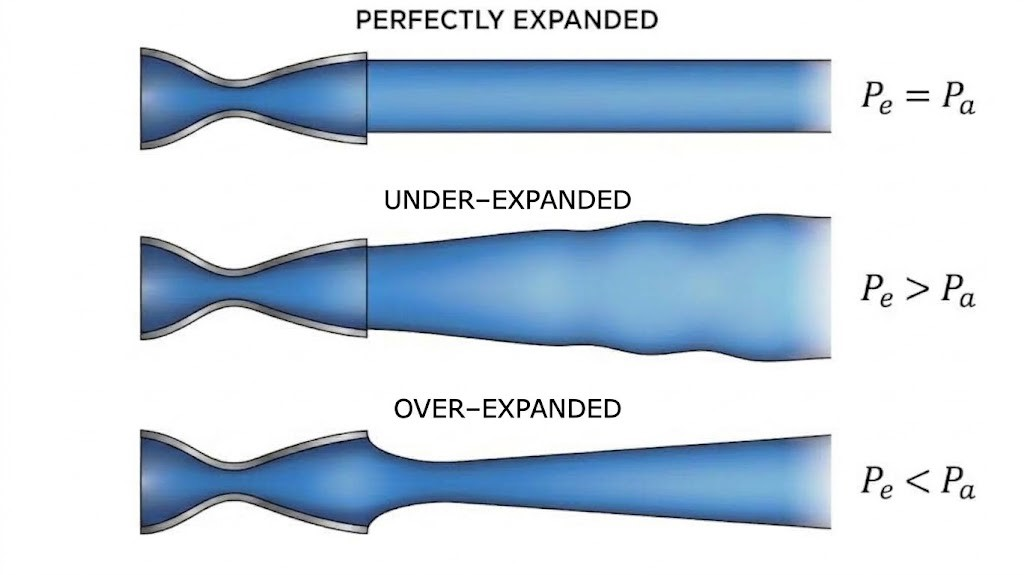
\includegraphics[width=0.8\textwidth]{figures/Under over and perfect expanded jets.jpg}
    \caption{Nozzle exit flow for the three expansion conditions: perfectly expanded ($p_e = p_a$), under-expanded ($p_e > p_a$) and over-expanded ($p_e < p_a$)}
    \label{fig: jet expansion regimes}
\end{figure}

\par Figure \ref{fig: planar underexpanded jet} shows the analytical solution of a planar under-expanded jet. It shows that the jet is marked by periodic structures called shock cells. These cells form as a mechanism of pressure adaptation between the nozzle exit and the ambient air through alternating Prandtl-Meyer expansion and compression waves \cite{vanHinsberg2014}. Since the the pressure at the nozzle exit is greater than the ambient pressure, the flow needs to expand to match the outside pressure. The results is a Prandtl-Meyer expansion fan anchored at the lip of the nozzle. These expansion waves are reflected at the axis of symmetry into another expansion fan, which in turn reflect at the jet boundary into compression waves. These converge into one another and coalesce, forming a shock. This shock increases the pressure, leading to another round of expansion waves. This process continues until, due to friction, the jet pressure equals the atmospheric pressure.


\begin{figure}[htbp]
    \centering
    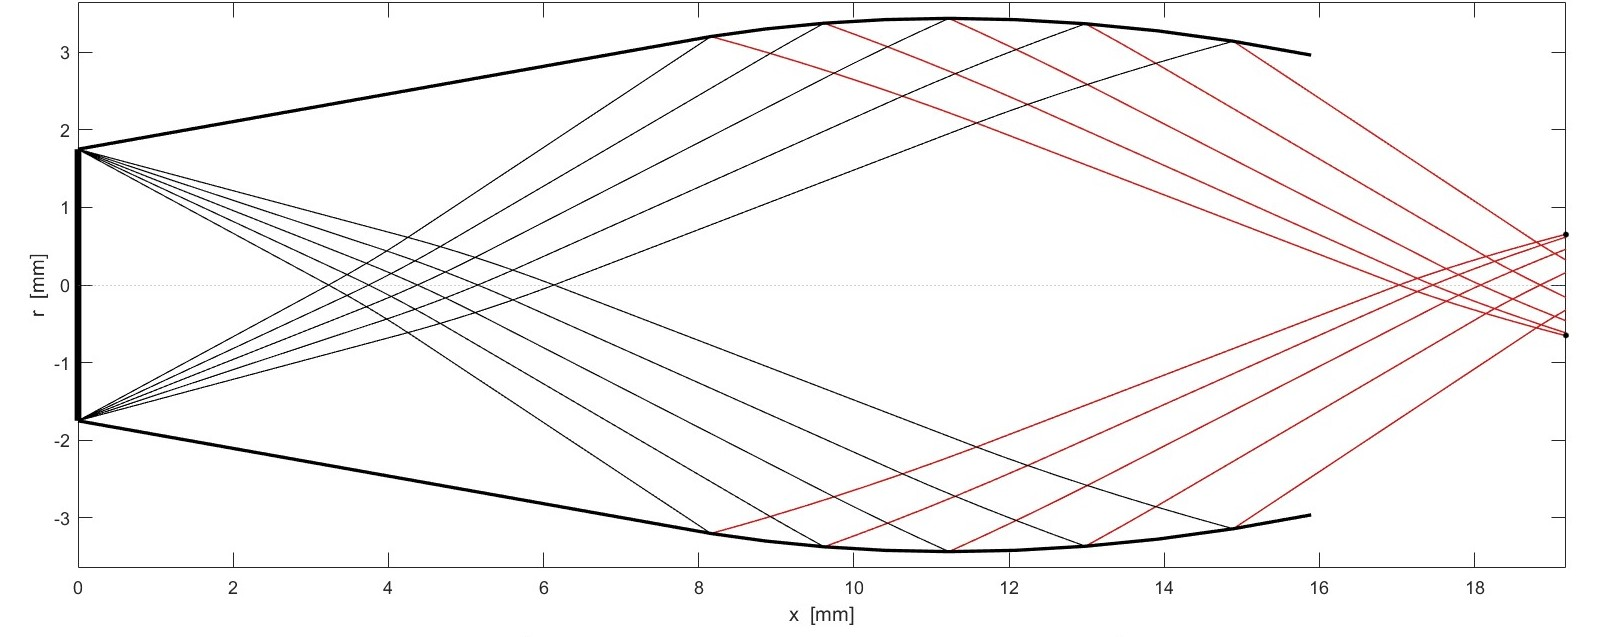
\includegraphics[width=\textwidth]{figures/under-expanded planar jet.jpg}
    \caption{Analytical solution of a planar under-expanded jet obtained using the Method of Characteristics with $M_e = 2$ and $p_e = 2 \cdot p_\infty$. The expansion waves leaving the nozzle lips (black) cross at the axis of symmetry, reflect at the jet boundary and return as compression waves (red), which converge and coalesce into a shock in the black dots at x= $19$mm}
    \label{fig: planar underexpanded jet}
\end{figure}

The three Figures \ref{fig: moderately underexpanded jet}, \ref{fig: highly underexpanded jet} and \ref{fig: unique barrel underexpanded jet} show sketches of under-expanded circular jets at different NPRs \cite{Duronio2023}. Due to it's axissymetry, the circular jet has a different structure to the planar case, displaying an early formation of an oblique shock extending from the lip to the jet axis, often called \emph{Intercepting shock}. When the NPR is between 2 and 4, as in Figure \ref{fig: moderately underexpanded jet}, this oblique shock reflects at the jet axis and goes to the shear layer, where it turns into an expansion fan, thus forming an "X" shape at each shock cell. For higher NPRs between 4 and 7, Figure \ref{fig: highly underexpanded jet}, the intercepting shock transitions to a singular reflection and produces a normal shock called \emph{Mach disk}, which gives each shock cell a "barrel" shape. For even higher NPRs, Figure \ref{fig: unique barrel underexpanded jet}, the jet is dominated by a single barrel. The last case is marked by a decreased jet boundary diameter and a very long plume caused by entraining air.

\begin{figure}[htbp]
    \centering
    \begin{subfigure}[b]{0.32\textwidth}
        \centering
        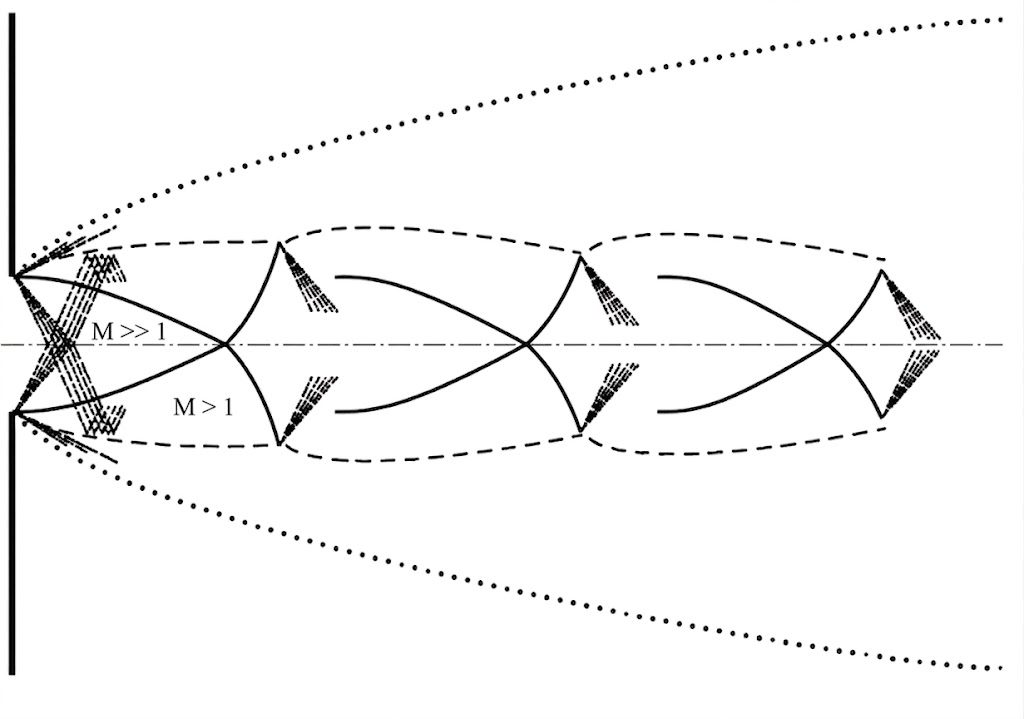
\includegraphics[width=\textwidth]{figures/moderately under-expanded jet.jpg}
        \caption{Moderately under-expanded, $2 < NPR < 4$}
        \label{fig: moderately underexpanded jet}
    \end{subfigure}
    \hfill
    \begin{subfigure}[b]{0.32\textwidth}
        \centering
        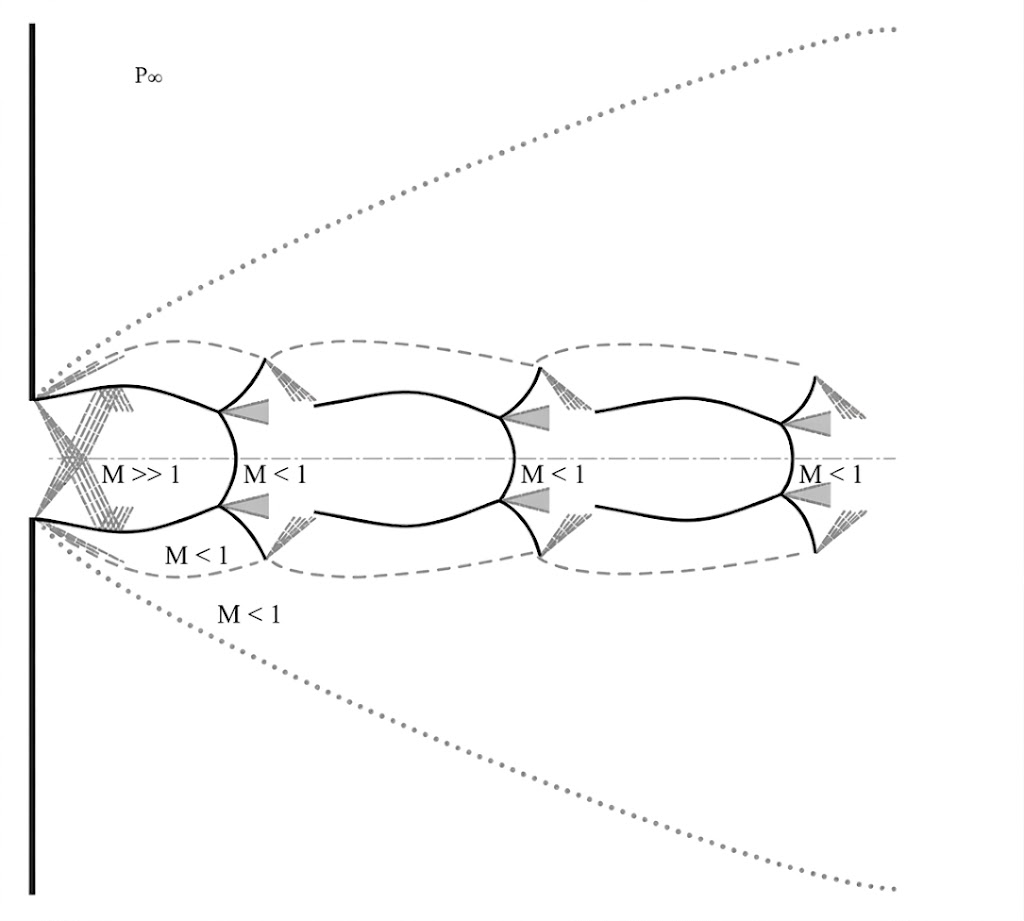
\includegraphics[width=\textwidth]{figures/highly under-expanded jet.jpg}
        \caption{Highly under-expanded, $4 < NPR < 7$}
        \label{fig: highly underexpanded jet}
    \end{subfigure}
    \hfill
    \begin{subfigure}[b]{0.32\textwidth}
        \centering
        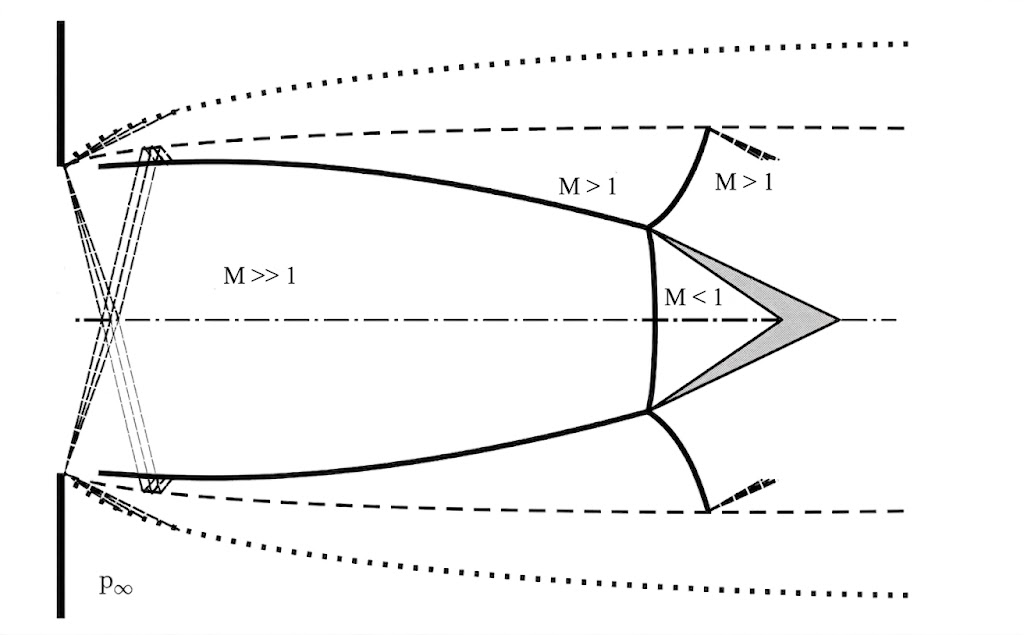
\includegraphics[width=\textwidth]{figures/unique barrel under-expanded jet.jpg}
        \caption{Single Barrel Structure, $NPR > 7$}
        \label{fig: unique barrel underexpanded jet}
    \end{subfigure}
    \caption{Sketches of circular under-expanded jets at increasing nozzle pressure ratio, credit to Duronio et al. \cite{Duronio2023}}
    \label{fig: circular underexpanded jets}
\end{figure}

As hinted by the scale of the sketches in Figure \ref{fig: circular underexpanded jets}, the $NPR$  also changes the length of the shock cells, $L_s$. Robert Emden was the first to correlate a weighted average of the $L_s$ of under-expanded choked jets with the $NPR$ in 1899 \cite{Powell2010, Emden1899}. After a series of experiments he reached the format of equation \ref{equation: Emden Formula}, where $k$ is a numerical coefficient that varies with the nozzle geometry and NPR range. The value of $k$ changed from 0.77 to 1.02 during the campaign, so Emden averaged the results of different nozzles to obtain $k = 0.88$. Later, Hartmann \& Lazarus \cite{Hartmann1941} used Emden's format with the average of all the cells except the first, achieving $k = 1.07$. They also correlated only the first shock cell length and introduced a constant term independent of $NPR$, obtaining the format of equation \ref{equation: Lazarus-Hartmann Formula}, with $a = 0.98$ and $b = 0.3$.
\begin{equation}
    \label{equation: Emden Formula}
    \frac{L_s}{d_N} = k\sqrt{NPR - NPR_c}
\end{equation}

\begin{equation}
    \label{equation: Lazarus-Hartmann Formula}
    \frac{L_s}{d_N} = a\sqrt{NPR - NPR_c}+b
\end{equation}

A circular jet created by a choked duct will be used to attest the capabilities of SBOS in producing a quantitative density field. In that context, this knowledge on axissymetric jet structure will be important to visually interpret the results after the experimental campaign. Furthermore, similar structures to those explained here for are present in different other applications, such as an aerospike nozzle. The next subsection will give a brief summary of the flow through a linear arospike nozzle and use much of what has been said here for that purpose.

\section{Aerospike Nozzle Flow}
\label{section: aerospike nozzle theory}
The distinct feature of an aerospike nozzle is the presence of its ramp right after its  exhaust. The ramp is designed so that the expansion fan anchored at the outside lip is not disturbed by the reflection of its own waves \cite{Wisse2005}. In the design condition, the flow expands through these waves, accelerating and reducing its static pressure, until design conditions are met, $M_{design}$ and $(p/p_a)_{design}$. In under-expanded condition, the same pressure adaptation process that happened in the free under-expanded jet now occurs in the ramp, where the flow is redirected to be parallel to the centerline. The result is a passive pressure adaptation mechanism that allows an aerospike to keep its thrust efficiency for a wide range of ambient pressures. In over-expanded condition, the flow is expanded below ambient pressure, the maximum turning angle of the fan increases, redirecting part of the exhaust flow sideways. Also, a shock may appear downstream so that ambient pressure is reached. Both mechanisms lead to a loss in thrust efficiency, so engineers try to avoid this condition and favor under-expanded and perfectly expanded flow. Figure \ref{fig: aerospike expansion regimes} shows the flow structure of an aerospike in under, perfectly and over expanded conditions.

\begin{figure}[htbp]
    \centering
    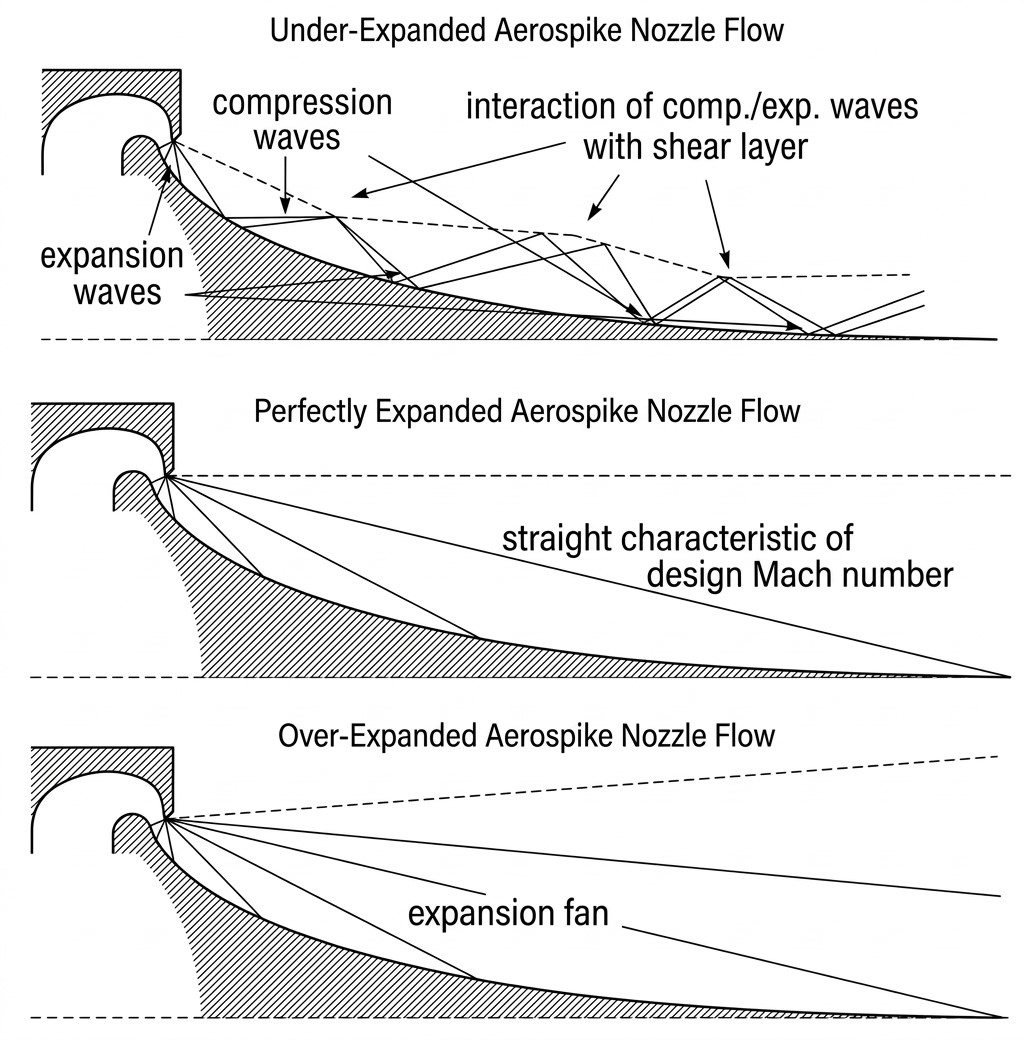
\includegraphics[width=0.6\textwidth]{figures/under perfect and over expanded aerospike.jpg}
    \caption{Flow structure of a linear aerospike nozzle in under-expanded, perfectly expanded and over-expanded conditions, credit to Wisse \cite{Wisse2005}}
    \label{fig: aerospike expansion regimes}
\end{figure}

It's the pressure adaptation feature present in an aerospike at under-expanded condition that makes it interesting for Single Stage to Orbit (SSTO) vehicles \cite{Wisse2005}. As shown in Figure \ref{fig: aerospike expansion regimes}, the process resembles the succession of expansion and compression waves present in the free under-expanded jet of Figure \ref{fig: planar underexpanded jet}. The mechanism always begins with an expansion wave at the outside lip of the exhaust exit. These waves reach the ramp and due to its concave geometry, the flow is compressed and reflect as compression waves. In the shear layer, the compression waves reflect into waves of other type and are redirected to the ramp. At this stage however, the curvature of the ramp is less accentuated and the waves reflect at the ramp to ones of the same family. The process continues with waves changing its type at the jet boundary and maintaining it when hitting the ramp, gradually fluctuating the ramp pressure around ambient conditions. This way, the flow is directed to be parallel to the centerline and there are no abrupt pressure differences capable of producing strong loss inducing shocks.

%The flow through the ramp of an aerospike nozzle will be investigated later using SBOS as a demonstration of the imaging method capabilities

The flow through the ramp of an aerospike nozzle will be investigated later using SBOS  to assess if the method has sufficient resolution and sensitivity to correctly study such complex flow field . In that context, the description of the flow physics will be of utmost important to assess if the method has sufficient resolution and sensitivity to correctly study the application. It is now clear from the previous sections how high-speeds and geometry leads to different flow structures that vary the fluid's density. The next section will explain how density influences the bending of light moving through a fluid, which is the fundamental principle behind optical density measurement techniques.

\section{Refraction}
\label{section: Refraction}
\par Refraction is the change in direction of a light ray as it propagates through a medium with spatially varying refractive index. This index is the ratio between the speed of light through vacuum, $c_0 \approx 3 \cdot 10^8$ m/s, and the speed of light through the medium, $c: n=c_0/c$.

\par The refractive index is a function of the light’s wavelength $\lambda$, and the thermochemical state of the environment it passes through. If $n$ is known at a certain wavelength and thermochemical state, it can be extrapolated to other states through the Lorentz-Lorentz equation, where $A$ is the molar refractivity, dependent on the wavelength, and $W_M$ the mean molecular weight \cite{Schmidt2025}.

\begin{equation}
    \frac{n^2 - 1}{\rho \left(n^2 + 2\right)}
=
\frac{A}{W_M}
=
\text{constant}
\end{equation}

\par The Gladstone-Dale is the linearization of this relationship for gases, where $n$ is almost 1 \cite{Head2021}. 

\begin{equation}
    n = 1 + G \rho
\end{equation}

\par This relationship directly links density with the refractive index, which in turn can be given by the distortion of light through the medium. $G$ is the Gladstone-Dale coefficient \cite{Head2021} \cite{Settles2001}.

\par As shown in Figure \ref{fig: Diagrams of light refraction}, when light passes from one medium to another it can behave differently depending on the refractive index field of the subsequent medium. The light’s interaction between two homogeneous media, shown in Figure \ref{fig: Diagrams of light refraction}a, is given by Snell’s Law of Refraction.

\begin{equation}
    n_1 \sin{\varepsilon_1} = n_2 \sin{\varepsilon_2}
\end{equation}

\begin{figure}[htbp]
    \centering
    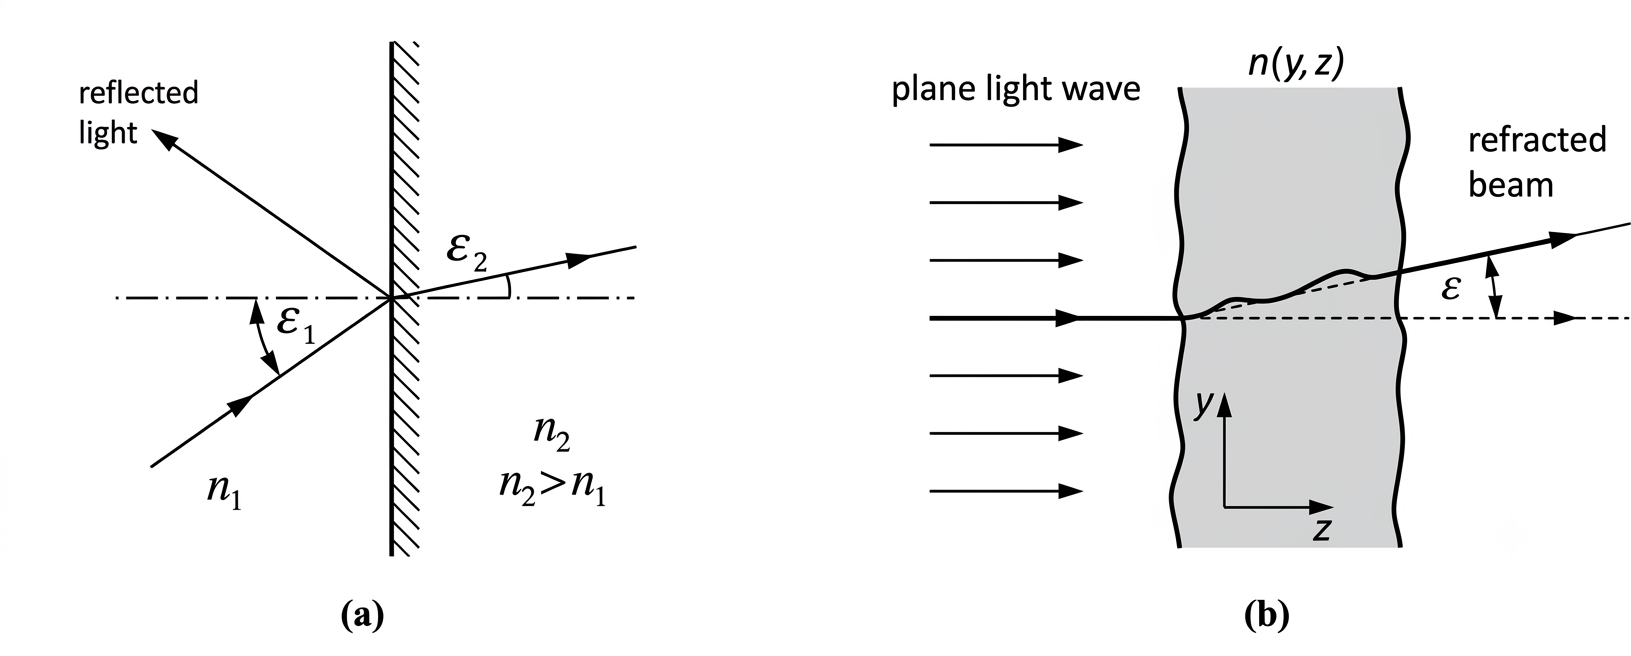
\includegraphics[width=0.8\textwidth]{figures/Diagrams of light refraction.png}
    \caption{Diagrams of Light refraction: (a) Change in the beam's direction between two homogeneous media as described by Snell's Law and (b) light refraction through an irregularly distributed refractive index environment. Credit to Schmidt et al. \cite{Schmidt2025}}
    \label{fig: Diagrams of light refraction}
\end{figure}

\par However, for inhomogeneous environments, as in Figure \ref{fig: Diagrams of light refraction}b, the change in light’s direction is not discrete. So a generalization must be performed to relate the deflection $\varepsilon$ to the refractive index field. Assuming small angle deflection and small refractive index gradient, the equation below is obtained, with $z$ being the line-of-sight direction \cite{Settles2001}.

\begin{equation}
    d\varepsilon_x = \frac{1}{n_o}\frac{\partial n}{\partial x}\,dz
\end{equation}

\par The total deflection is the integral of $d\varepsilon$ along the ray path, as is shown below. An analogous equation exists for $y$, by substituting it in $x$.

\begin{equation}
\label{equation: displacement integral}
    \varepsilon_x
=
\frac{1}{n_o}
\int \frac{\partial n}{\partial x} dz
\end{equation}

\par Now, if a substitution is applied with the Gladstone-Dale relationship, one can obtain:

\begin{equation}
\label{equation:epsilon-nabla rho}
    \vec{\varepsilon}
=
\frac{G}{n_o}
\int \nabla \rho \, dz
\end{equation}

\par Equation \ref{equation:epsilon-nabla rho} links directly the light deviation vector to the density gradient through media. Thus, in order to obtain a quantitative measure of the density field through a test section, one could employ a method to measure the displacement of light after passing through it. If the transversal refractive gradients are independent to the line of sight direction, such as a 2D planar flow, Equation \ref{equation:epsilon-nabla rho} can be simplified into Equation \ref{equation: Displacement and Density Gradient} for $x$, where $W$ is the refractive object thickness \cite{RajendranDotTracking}.

\begin{equation}
    \label{equation: Displacement and Density Gradient}
    \varepsilon_x = \frac{G\cdot W}{n_0} \frac{\partial \rho}{\partial x}
\end{equation}

The equation shows that light bends in the direction of the desnity gradient, that is, the direction of highest density. For a 2D planar flow, if the displacements caused by light passing through it are measured in a plane, the object density gradient can be computed and integrated to obtain a density field. For a more complex 3D flow, multiple line of-sights must be used to reconstruct a tomographic image of the density. However, some 3D flows can be reconstructed with only a 2D view due to it's symmetry. An axissymetric body is one of such case which occur frequently in various applications. The next section will demonstrate how axissymetry can be used to obtain the 3D density field using 2D displacement vectors.

\subsection{Axisymmetric Refractive Field}
\label{subsection: Axisymmetric Refractive Field}

When a refractive object is axially symmetric, it is possible to reconstruct its whole density distribution with only a 2D snapshot of the light displacements through it. In such scenario, the image is a 2D projection of a 3D axisymmetric body, and the inverse Abel transform can be used to obtain its radial and axial profile \cite{Abel1826}. Consider the case in Figure \ref{fig: Abel transform} and Equation \ref{equation: displacement integral} for y, it can be integrated in y in both sides into Equation \ref{equation: integral of epsilon}, which removes the partial derivative through the fundamental theorem of calculus.

\begin{figure}[h]
    \centering
    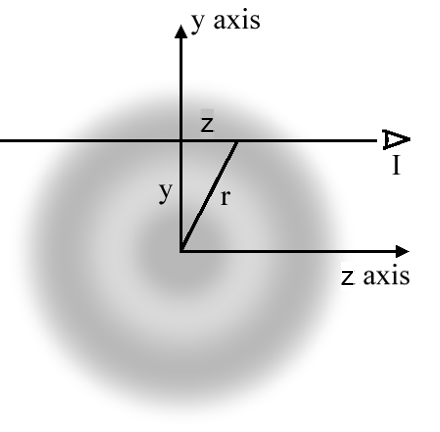
\includegraphics[width=0.3\textwidth]{figures/AbelTransform.png}
    \caption{Diagram of the geometry of an axisymmetric body being seen by an observer in I. If the body, in grey, is described by a function $f(r)$, the observer will see its projection $F(y)$, which is its Abel transform}
    \label{fig: Abel transform}
\end{figure}

\begin{equation}
\label{equation: integral of epsilon }
    E_y = \frac{2}{n_0}\int_0^R [n(r) - n_0]dz
\end{equation}

Now, by changing $z$ for the radius $r$, $E_y$ becomes the plain Abel transform of the refractive index $n$ in Equation \ref{equation: Abel transform of n}. This means that when the inverse Abel transformation is applied to $E_y$, a radial profile of $n$ is obtained, which can be translated to the density through the Gladstone-Dale relation.

\begin{equation}
    \label{equation: Abel transform of n}
    E_y = \frac{2}{n_0} \int_0^R \frac{[n(r) - n_0]}{\sqrt{r^2-y^2}}r dr
\end{equation}

This chapter has shown how changes in density can emerge in different flow conditions and how these variations modify the flow's refractive properties. It is the ability to relate optical distortions to density gradients that forms the foundation of schlieren-based diagnostic techniques. The next chapter will treat these methods by presenting a brief history of how researchers have been able to measure the bending of light and translate it into qualitative and quantitative thermodynamic measures over the years, culminating in the state of the art and the topic of this thesis, SBOS.